\chapter{Concept \label{chap:concept}}

%Big picture
%General ideas how to solve goals
%Present equal concepts with theoretical pro's and cons
%What are the general ideas that we try to solve the problem with?

In order to allow a robot to continuously %TODO...
Unlike in isolated classification or regression tasks, it is not enough to employ one specialized machine learning algorithm in order to solve the given problem. Since the model is supposed to interact with its environment and update itself while experiencing new interactions, a more important complex model is required. While the chosen underlying regression and classification methods need to fulfill certain conditions and greatly influence the resulting model performance, they could easily replaced by suitable alternatives. Even more important is the architecture around them, that organizes the information coming from the environment and adapts where necessary. This chapter presents the general concepts behind the two developed models and the way the information is organized.

First a more detailed specification about the problem is given in section \ref{sec:problem}. Afterwards,
section \ref{sec:pairInt} describes the first developed concepts working solely in what is called the interaction space in this thesis. The alternative approach of modeling object states directly is described in section \ref{sec:gate}.

\section{Problem specification \label{sec:problem}}

As stated in the introduction, the goal of this thesis is to provide possible models that incrementally learn simple interactions between physical objects. Without any training the model should be able to interact with the environment as visualized in figure \ref{fig:overview}. %TODO pushing contacts not really correct, sounds like I only deal with the moments where they are already connected
One object, the actuator, can be controlled by the model through known action primitives. The results of these actions however are not necessarily known to the model beforehand. Consequently, the model might be required to learn a forward model of its actuator as well as the pushing interactions. Apart from the actuator at least one more object is present in the environment. Given a certain state of the environment and a selected action primitive, the model is supposed to make accurate predictions about the state of the environment after the action has been performed. Since the actuator, or some other object, might push objects that are not directly controllable through actions, the state of all objects in the scene need to be predicted. 

Furthermore, when a specific target state for an object is given, the inverse model should select an action primitive, that will bring the objects in the environment closer to the target state. The inverse model needs to include the pushing interactions, since only the actuator can be controlled directly. It might be required to bring the actuator in a suitable position before another object can be pushed in the correct direction. %TODO sounds strange

\begin{figure}
	\centering
	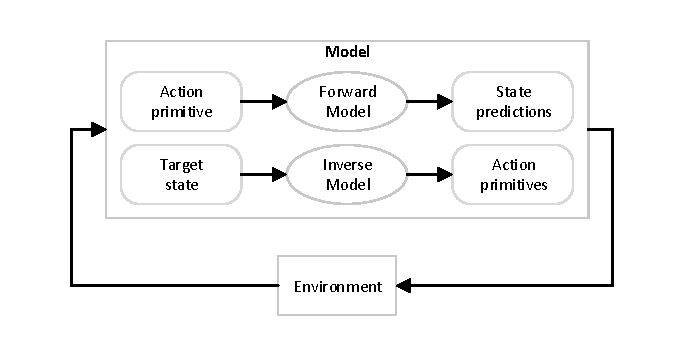
\includegraphics{Overview.pdf}
	\caption{Overview of the problem. The model includes a forward model in order to make predictions given the current environment state and a certain action primitive. When given a target state the inverse model provides suitable action primitives to reach the desired state.}
	\label{fig:overview}
\end{figure}

\section{Modeling pairwise interactions \label{sec:pairInt}}

The first approach tries to find distinct subspaces in the \textit{interaction space} between two objects. In this context, the interaction space represents the space of all interactions between two objects. This includes their relative placement and movement to each other, as well as their influence, for example by pushing, on each other. Instead of modeling and learning forward and inverse models for each object, only the pairwise interaction space between two objects is considered.  

For every object pair an \textit{interaction state} is considered. This interaction state represents one object's state relative to the second object's state. This includes for example transforming each objects position and orientation to the local coordinate system of the second object. %For the realization, described in section \ref{sec:pairRealization}, he actuator is not used as reference.
The predicted object states are extracted from the predicted interaction states.

At each update step the current interaction states for all object pairs in the environment are received. The previous state, the performed action and the resulting state are collected and stored as an \textit{episode}. The general idea is to store these episodes as past knowledge similar to the approach in case based reasoning \cite{cbr}. When predicting, these episodes can be searched for the most similar one. The similarity can be determined by comparing the previous state of each episode to the given interaction state and the used action to the current action:

\begin{equation}
	e^{best} = \argmin_{e^i \in E} ||e^i_{preState}-curState, e^i_{action}-curAction||_e
	\label{eq:bestEpisode}
\end{equation}


$e^i$ represents the i's episode that has been stored yet. $e^i_{preState}$ means only the previous interaction state of the episode, while $e^i_{action}$ represents the used action in that episode.
The norm $||a,b||_e$ is a special norm used to allow different weighting of the features from the previous state and the action. For planning, the action difference can be swapped with the difference between the resulting state of each episode and the desired target state.

Once the most similar episode has been found, the desired information can be extracted from it. That is the resulting state for prediction or the action for planning. The formula above represents a nearest neighbor search on all episodes. Although such an approach can work, it quickly becomes infeasible when the number of stored episode keeps growing. Since the nearest neighbor search scales linearly with the number of stored examples it is unsuitable for lifelong learning. 

As mentioned above, the idea of this concept is to split the interaction space into subspaces and train local models for each of these subspaces. An overview of the structure can be seen in figure \ref{fig:PairOverview}.
The episodes corresponding to the same subspace are collected in \textit{abstract collections} which are further explained in section \ref{sec:ACs}.
The \textit{Abstract Collection Selector} is needed in order to choose the most appropriate abstract collection in a given situation. The realization of this concept is described in section \ref{sec:pairRealization}.

\begin{figure}
	\centering
	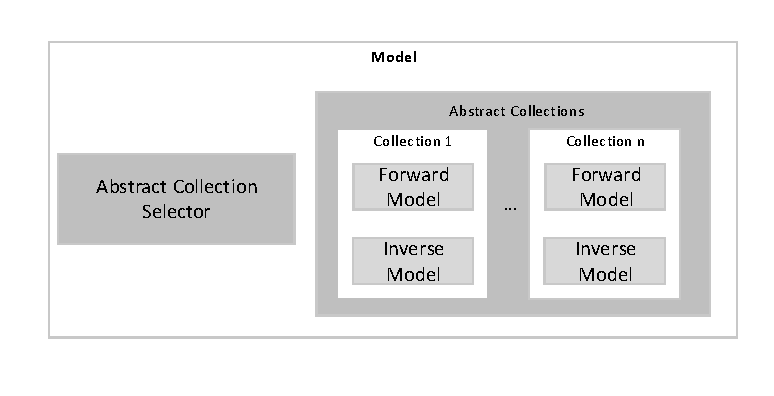
\includegraphics{PairwiseOverview.pdf}
	\caption{Overview of the model in interaction space. The different abstract collections contain forward and inverse models of distinct subspaces of the interaction space. The selector is needed in order to select the correct submodel for prediction. TODO consider adding transformation to interaction state and back to object states as well?} %TODO
	\label{fig:PairOverview}
\end{figure}

\subsection{Abstract collection \label{sec:ACs}}

The clustering of episodes suggested here is based on the set of attributes that changed between the previous state and the resulting state while performing an action. The set $S$ of attributes that changed is defined as follows 
\begin{equation}
S = \{f | f \in F ~ \wedge ~ ||Pre(f)-Post(f)|| > \epsilon_{Noise}\}
\end{equation}
where $F$ denotes the set of all features, $Pre(f), Post(f)$, the value of 
feature $f$ in the initial and resulting state of the episode respectively and 
$\epsilon_{Noise}$ a threshold to cancel out small noise.

Each different set is represented by a different abstract collection $AC_i$. The 
idea is that these collections correspond to different interaction scenarios.
Consider an exemplary interaction state with the named attributes distance and angle.
The distance represents the closest distance between the two objects represented by the interaction state. The angle gives the angular direction the second object is located with respect to the local coordinate system of the reference object. The set containing only the distance represents all interactions where one object moves straight towards or away from the other object. The set where nothing changes would signal a pushing interaction, when an action is being performed.

Since each distinct interaction scenario results in a different set of changing attributes, the interaction space is split into subspaces by these collections. The resulting collections create an abstract representation for each of these interaction scenarios.

These collections can then train their respective local forward and inverse models. These can be simple nearest neighbor structures as mentioned above. Alternatively, any suitable regression model can be trained. Depending on the model this can reduce the amount of episodes that need to be stored as well. Furthermore, each collection can perform local optimizations such as automatic feature selection.

\subsection{Prediction}
%TODO consider removing DT here, since it is not used anymore and was never as good as what we have now
The general idea for prediction within this concept is visualized in figure \ref{fig:PairPrediction}. As mentioned above, the interaction state is computed first.
Afterwards, the collection that is most likely 
responsible for the next episode is estimated. This estimation is performed by the Abstract Collection Selector. This selector can be a classifier, e.g. a decision tree \cite{DT}, trained on all the input-collection pairs. Such a classifier brings the advantage that the selection becomes 
independent of the amount of episodes already stored. The total number 
of collections is limited to the size of the superset of $F$, although in 
practice, not all possibilities are likely and only those collections are 
considered, that are already made up of more than $\epsilon_{min}$ training 
examples. This threshold is used to reduce the number of outliers when training the 
classifier.  

After the suitable abstract collection has been selected, its forward model can be consulted for the prediction. This results in a predicted interaction state. The respective object states need to be extracted from this by reverting the transformations again.

\begin{figure}
	\centering
	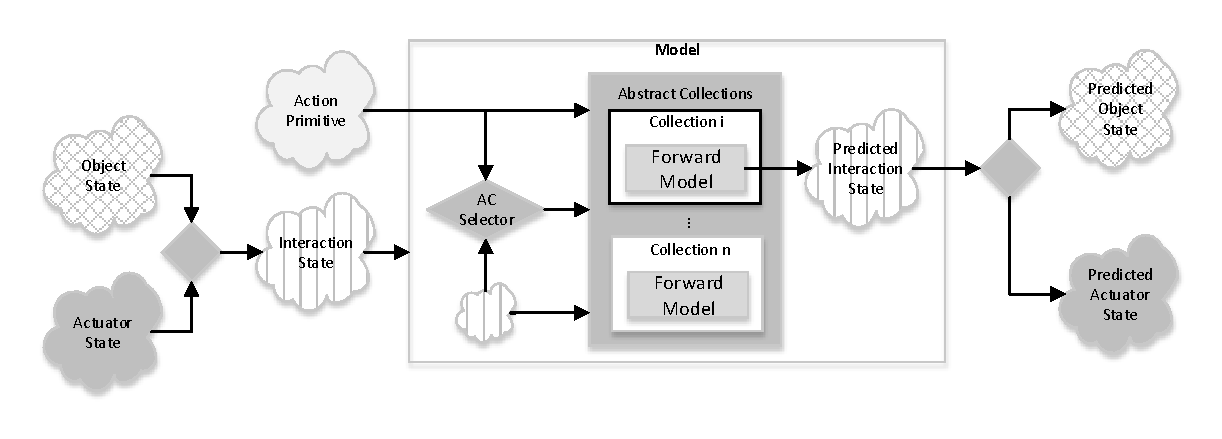
\includegraphics[width=\textwidth]{PairwisePrediction.pdf}
	\caption{Concept of prediction in the pairwise interaction space with abstract collections. First the interaction state is computed. This state is then fed to the model which uses it to select the responsible abstract collection with the selector (AC Selector). The collection then uses its forward model to predict the next interaction state. The actual predicted object states are finally extracted from this interaction state.} 
	\label{fig:PairPrediction}
\end{figure}

\subsection{Planning}

%TODO
(TODO consider redoing the planning algorithm more similar to the way it is done
in the most recent model, which works, maybe the same ideas can be employed 
here)

In order to get a suitable action given a target configuration, first the 
difference set between the current situation and the target 
configuration is computed. Afterwards, the abstract collection that corresponds to the same set of attributes. In case such a collection is not yet known, the 
most similar collection is chosen instead. This is the collection that covers 
most of the changed attributes in the computed difference set. 

The selected abstract collection queries its own inverse model for the 
action that produces the output most similar to the desired target configuration. 

The action is then checked by consulting already trained forward models. In case the forward models predict that the selected action does not reduce the difference to the target, a different action needs to be selected. This is done by querying a different abstract collection. Alternatively, a random action can be performed in order to produce new episodes. These in turn would improve both the forward as well as the inverse models of their respective abstract collections.

\subsection{Theoretical discussion}

Using pairwise interaction states in order to represent the interactions between objects is often used in robotics, for example in \cite{pairwiseExample}. Its advantage is that it represents both objects involved in an interaction at the same time. In theory this should make it less likely that impossible configurations are predicted such as solid objects being inside of each other. Furthermore, such an interaction state can contain all the necessary information about the objects in one representation. 

The downside of this approach is that the actual object states need to be inferred from these interaction states. While this will only involve simple coordinate transformations in most cases, some object attributes might not be as easily transformable. Furthermore, in order to contain all the necessary information about both objects, these interaction states can become fairly high dimensional. 

An even bigger disadvantage is the fact that only pairwise interactions are represented. When considering environments with more than two objects, interactions between three objects are not represented. Predictions of an object that is involved in two pairwise interactions can vary greatly and it is difficult to say which prediction, if any is accurate.

\section{Object space with gate \label{sec:gate}}

The alternative to modeling only the interaction space, is to model each object and perform predictions for each object separately. The general components of this concept is visualized in figure \ref{fig:gateOverview}.
The idea is to train local forward and inverse models for each object, or object group in the \textit{Predictor}. %TODO consider changing this name
An object group can be considered a collection of objects that are similar in the way they behave during interactions. Therefore they can be represented by a single local model. One example would be two identically shaped block objects that only have different colors. In order to detect if two objects should be grouped together or not, one can start with training separate local models and compare their outputs. If two models appear to be similar, they can be merged together. Ideally, a similarity measure for objects is provided. Following the assumption that similar objects should behave similarly, such a measure would allow the grouping from the start. 

The \textit{Gate} learns a classifier in order to distinguish interactions between objects from no interactions. While in the previous concept everything was treated as an interaction, this idea only considers instances as interactions where one object actually influences another directly. Furthermore, this idea assumes, that object states do not change without any interaction. The only exception is the \textit{Actuator}. Here, the actuator is treated as a special kind of object with its own forward and inverse model. These models can be provided beforehand or learned online. 
The gate allows that the local forward and inverse models are only trained and tested in instances where there actually is interaction. Similar to the previous concept, this creates a subspace in the entire interaction space introduced before. The local models require less training data that way since they do not need to cover the entire interaction space. 

The current state of each object, including the actuator, is always updated when new information is received from the environment. At each update the gate and, if required the actuator's local models are trained. On top of that, the local models responsible for any object whose state changed with the last update, are trained as well.


\begin{figure}
	\centering
	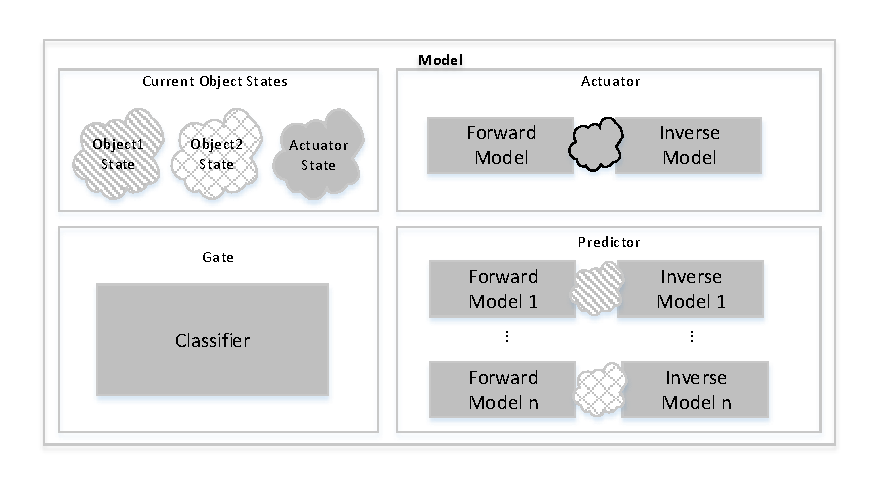
\includegraphics{GateOverview.pdf}
	\caption{Overview of the concept about object state with gate. The actuator is a special object, that can be influenced directly. It's forward and inverse model might even be provided if known. For the other objects/object groups, the Predictor learns these models. The Gate learns a classifier to distinguish interactions between objects from only single object changes.} 
	\label{fig:GateOverview}
\end{figure}

\subsection{Prediction}

Because of the assumption that objects other than the actuator cannot change without any interaction, the way prediction is performed differs between the different object types. The actuator simply queries its own forward model with the selected action primitive in order to predict the next actuator state. 

In order to predict interactions, that means changes in the state of any non actuator object, the process visualized in figure \ref{fig:GatePrediction} is used.

\begin{figure}
	\centering
	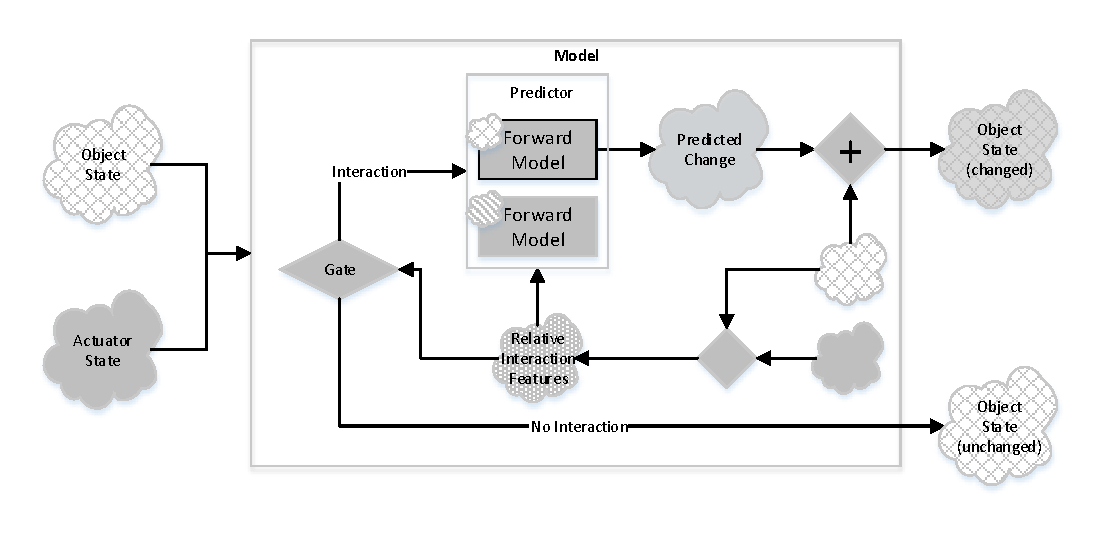
\includegraphics[width=\textwidth]{GatePrediction.pdf}
	\caption{Visualization of the prediction process for non actuator objects in the object space with gating concept. Using the predicted actuator state, relative interaction features are computed. These are used by the gate to determine if an interaction takes place or not. The responsible local forward model is used to predict the changes if an interaction is expected. From these changes the actual state prediction is computed.} 
	\label{fig:GatePrediction}
\end{figure}

First the next actuator state is predicted as mentioned above using the selection action primitive.
This prediction along with the current object state of the object that is to be predicted is used to compute \textit{Relative Interaction Features}. These relative features are similar to the interaction state that was explained in the previous concept. However, since it is not necessary to extract the entire object states for both objects from these relative features, the dimensionality can be a lot lower than before. These features are then used to first determine if the current object is actually part of an interaction with the actuator. If the gate predicts no interaction between the object and the actuator, the current object state is returned. 

On the other hand, if an interaction is predicted, the Predictor uses the relative features to query the local forward model responsible for the current object to make a prediction. The local model predict the changes in the object states instead of the final states. This allows the local models to be independent of the actual object states. This assumes, that an interaction between two objects behaves the same in different situations as long as their relative interaction features are the same. In order to get the actual predicted object state, these changes are added to the current object state.

When more then one object apart from the actuator is present, the same process can be repeated. In order to predict interactions between two non actuator objects, a prediction chain is performed. First the actuator is predicted as described above. Afterwards, the objects that are directly influenced by the actuator are predicted. These predictions can then in turn be used as new \enquote{actuators} for interactions between them and other objects. 

%TODO decide which is used
%(STILL TO TRY) In order to predict multi object interactions, the gate function can be used to first collect all involved objects before
%invoking the appropriate predictor. (e.g. by interpolating the different input features).

\subsection{Planning}

Similar to prediction, planning is also performed differently depending on what kind of object is supposed to reach some target configuration. In the case that the target object is the actuator, its inverse model is queried for an action primitive given the target configuration. 

The more interesting process of reaching a target configuration for a non actuator object is visualized in figure \ref{fig:GatePlanning}.

\begin{figure}
	\centering
	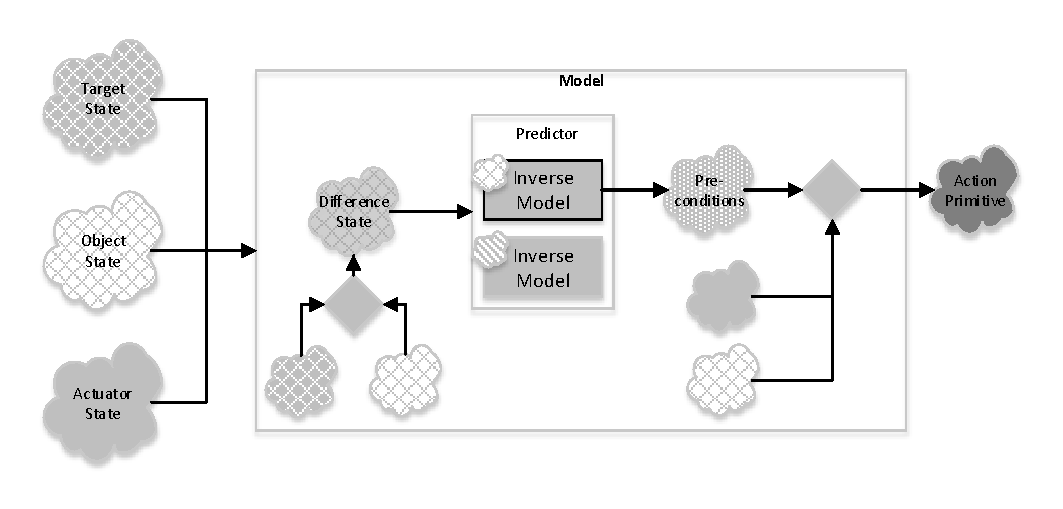
\includegraphics[width=\textwidth]{GatePlanning.pdf}
	\caption{Visualization of the planning process for non actuator objects in the object space with gating concept. } 
	\label{fig:GatePlanning}
\end{figure}

First the current difference state is computed from the given target configuration and the current object state. This difference state is then used to query the responsible inverse model. Since only the actuator can be influenced by actions directly, these local inverse models do not directly return action primitives. Instead they return preconditions in the form of the relative interaction features that result in a change that reduces the difference to the target configuration. The current actuator state is then compared to these preconditions. If the actuator is already in a configuration where it meets these preconditions, an action primitive can be derived from the local features. In most situations this will however not be the case. The given preconditions will often require the actuator to be in a different position relative to the object that is to be moved. In these cases, the suitable position for the actuator, is used as a intermediate target. Considering the current object's position, an action is calculated to move the actuator towards the intermediate target. This might result in a circling movement of the actuator around the object. Moving the actuator directly towards the intermediate target position, might result in moving the object in a more unfavorable position and is therefore avoided. Since these steps are performed at every timestep, the model can quickly adapt to changes in the environment.

%TODO
[TODO is this realization?]

For this concept, a special kind of inverse model was developed. Directly searching in the inverse regression model has several disadvantages in the given scenario: Firstly, the difference state that is computed can have features magnitudes greater than any change the local models have been trained with. The inverse model would need to extrapolate into unknown regions in these cases. Secondly, the features in the target state are not necessarily normalized. Therefore, the model does not necessarily know if a reduction of difference feature A by X at the cost of an increase of difference feature B by Y is better than the opposite. In the context of this thesis such a scenario is given by features representing position and orientation. 

In order to avoid these problems, the proposed inverse model ignores the actual quantity of a change. Instead, the inverse model focuses on the direction of the changes. A prototype is trained for each direction of each feature that changed in the object state during an update. Each prototype computes a weighted average of the preconditions that resulted in a feature change represented by it. The preconditions are weighted by the magnitude of the change. 

Simply taking the average is however not possible as can be seen in figure \ref{fig:avgProblem}.

\begin{figure}
	\centering
	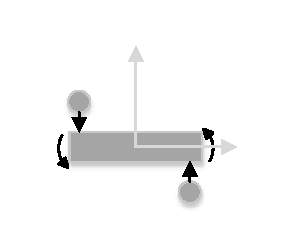
\includegraphics{avgProblem.pdf}
	\caption{Visualization of the averaging problem for point symmetric features. The circles represent the actuator while the rectangle represents a block object. Both pushing scenarios result in the same direction for orientation change of the object, however averaging the relative x and y positions would result in an invalid precondition.} 
	\label{fig:avgProblem}
\end{figure}

For point symmetric features, such as relative x and y positions in the figure, averaging results in invalid preconditions. In this case, the averaged preconditions would want the actuator to be in the center of the block, which is neither possible nor would it result in an orientation change. In order to prevent this, two averages are computed for each feature. One for all positive values of that feature and one for all negatives. on top of that, all combination of feature signs are stored and weighted by the magnitude of the change. When returning the entire preconditions, the averages corresponding to the sign combination with the highest weight are returned. Table \ref{tab:signCombinations} shows the combinations visible in the example above. In case combination 1 has the highest weight, the positive average for the x position, the negative average for the y position and the positive average for the y velocity is used. 

\begin{table}
	\centering
\begin{tabular}{|c|c|c|}
	\hline Feature & Combination 1 & Combination 2 \\ 
	\hline x position & + & - \\ 
	\hline y position & - & + \\ 
	\hline y velocity & + & - \\ 
	\hline 
\end{tabular} 
\caption{Table showing the sign combinations for the example in figure \ref{fig:avgProblem}}
\label{tab:signCombinations}
\end{table}

